%\documentclass{beamer}
\documentclass[handout]{beamer}
\usepackage[utf8]{inputenc}
\usepackage[T1]{fontenc}
\usepackage[francais]{babel}
\usepackage[babel=true]{csquotes}
\usepackage{dcolumn}
\usepackage{graphicx}
\usepackage{epsfig}
\usepackage{pgf}
\usepackage{pstricks}
\usepackage{pst-node}
\usepackage{listings, lstautogobble}
\usepackage{siunitx}
\graphicspath{{Images/}}
\newcolumntype{.}{D{.}{.}{-1}}
\newcolumntype{d}[1]{D{.}{.}{#1}}
\usetheme{Warsaw}

\setbeamertemplate{frametitle}[default][center]
\beamerdefaultoverlayspecification{<+->}

% couleur du texte pour java
\definecolor{mygreen}{rgb}{0,0.6,0}
\definecolor{mygrey}{rgb}{0.5,0.5,0.5}
\definecolor{mymauve}{rgb}{0.58,0,0.82}

\lstset{ %
  backgroundcolor=\color{white},   % choose the background color
  basicstyle=\fontsize{8}{11}\ttfamily,        % size of fonts used for the code
  breaklines=true,                 % automatic line breaking only at whitespace
  captionpos=b,                    % sets the caption-position to bottom
  commentstyle=\color{mygreen},    % comment style
  escapeinside={\%*}{*)},          % if you want to add LaTeX within your code
  keywordstyle=\color{blue},       % keyword style
  stringstyle=\color{mymauve},     % string literal style
  autogobble=true,                 % indentation automatique
  showstringspaces=false           % pas de caractères spéciaux pour les espaces
}

\newcommand{\norm}[1]{\lVert#1\rVert}


\title{Soutenance de Projet Android}
\author{Arthur Wenger \& Shad Maleck}
\date{\today}
\institute{\normalsize{M1 Informatique Université de la Réunion}}
\begin{document}

\begin{frame}
  \titlepage
\end{frame}

\begin{frame}
  \frametitle<1->{\center{Introduction}}
  \begin{block}<1->{Objectif}
    \begin{itemize}
    \item <1->{Créer un jeu simple sur Android}
    \end{itemize}
  \end{block}
    \begin{block}<2->{Contraintes}
    \begin{itemize}
    \item <2->{Utiliser un capteur pour déplacer une balle}
    \item <3->{Créer une liste de scores}
    \item <4->{Gérer la persistance des scores}
    \item <5->{Créer une carte pour visualiser les scores}
    \item <6->{Ajouter du son}
    \end{itemize}
  \end{block}
\end{frame}

\begin{frame}
  \frametitle<1->{\center{Présentation du jeu}}
\begin{block}<1->{Principe}
    \begin{itemize}
    \item <1->{Reprendre le concept de Pacman}
    \begin{center}
      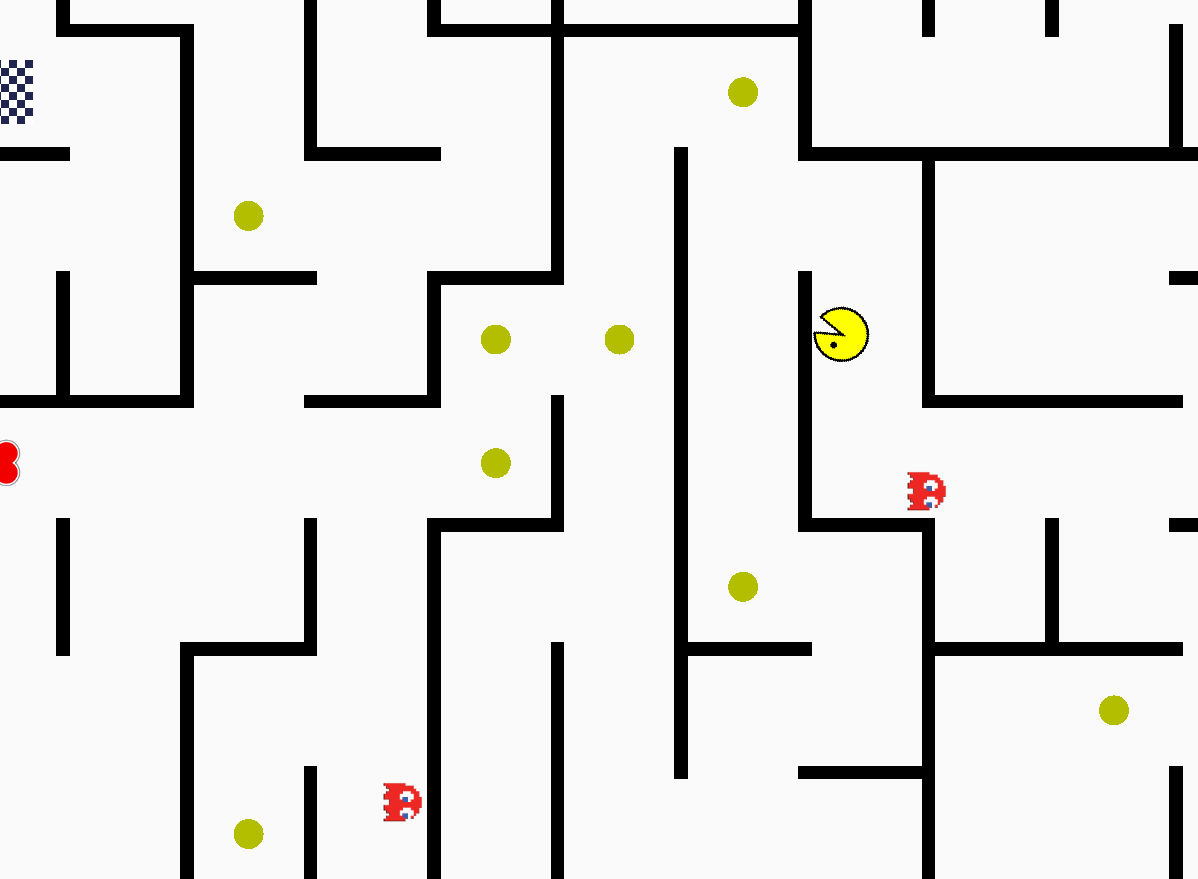
\includegraphics[width=40mm]{game_screen.png}
    \end{center}
    \end{itemize}
  \end{block}
  \begin{block}<2->{Implications}
    \begin{itemize}
    \item <2->{Créer un labyrinthe}
    \item <3->{Utiliser accéléromètre pour déplacer pacman}
    \item <4->{Gérer les collisions avec les murs et les objets du jeu}
    \end{itemize}
  \end{block}
\end{frame}

\begin{frame}
  \frametitle<1->{\center{L'accéleromètre}}
    \begin{itemize}
      %soustraction de la force de gravité => 9.1 m/s² au repos
      % P=mg d'ou : a = -P/m = -g au repos
    \item <1->{Mesure l'accélération de l'appareil selon 3 axes:}
    \begin{center}
      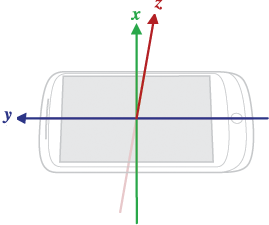
\includegraphics[height=30mm]{accelerometre.png}
    \end{center}
    \begin{center}
      $\vec{a_d} = - \frac{\sum \vec{F}}{m} - \vec{g}$ avec $\norm{\vec{g}} = \SI{9.81}{\meter\per\second\squared}$
    \end{center}

    \item <2->{Quand l'appareil ne bouge pas:}
    $\sum \vec{F} = 0 \implies \vec{a_d} = - \vec{g}$

    \item <4->{L'accélération détermine l'orientation du téléphone}

    \item <3->{Mais l'accélération est aussi une variation de vitesse:}% on peut donc l'utiliser pour déplacer Pacman
    \begin{center}
    $\vec{a} = \frac{{d\vec{\upsilon}}}{{dt}} = \frac{{d^2 \vec{x}}} {{dt^2 }}$
    \end{center}
    \end{itemize}
\end{frame}

\begin{frame}[fragile]
  \frametitle<1->{\center{Les mouvements de Pacman}}
    \begin{itemize}
    \item <1->{Capture et transmission de l'accélération:}%parler de sensor_delay_ui
    \begin{lstlisting}[language=java]
    manager.registerListener(sensorListener, mAccelerometer, SensorManager.SENSOR_DELAY_UI);

    private class MySensorListener implements SensorEventListener {
      public void onSensorChanged( SensorEvent event ) {
    if (event.sensor.getType()==Sensor.TYPE_ACCELEROMETER)
    mazeView.updateAccel(-event.values[0],event.values[1]);
    }}
    \end{lstlisting} % pas de "-" pour value[1] car on inverse l'axe y (inversion des x car a = -g)

    \item <2->{Mise à jour de l'accélération de pacman}
    \item <3->{Prise en compte de l'accélération en utilisant la formule:}
    $ v_f = v_i + a*dt $ avec $ dt = \frac{1}{FPS} $
    \end{itemize}
\end{frame}

\begin{frame}
  \frametitle<1->{\center{Le labyrinthe}}
    \begin{itemize}
    \item <1->{Génération aléatoire avec l'algorithme \enquote{Depth-first search}}
    \begin{figure}[htp]
      \centering
      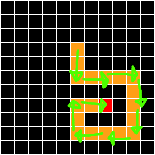
\includegraphics[width=.3\textwidth, height=30mm]{DFS1.png}\hfill
      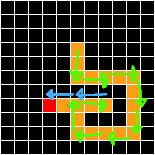
\includegraphics[width=.3\textwidth, height=30mm]{DFS2.png}\hfill
      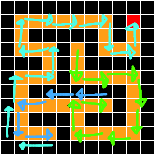
\includegraphics[width=.3\textwidth, height=30mm]{DFS3.png}
    \end{figure}
    \item <2->{Création des murs avec une classe modélisant un segment}
    \item <3->{Initialisation des positions des objets du jeu}
    \end{itemize}
\end{frame}

\begin{frame}
  \frametitle<1->{\center{La vue et les objets du jeu}}
  \begin{block}<1->{La vue}
    \begin{itemize}
    \item <1->{Une vue spécifique \enquote{GameView} }
    \item <2->{La méthode onDraw pour dessiner le labyrinthe et les objets}
    \item <3->{Un thread pour mettre à jour le jeu}
    \end{itemize}
  \end{block}
  \begin{block}<2->{Les objets}
    \begin{itemize}
    \item <4->{Des sprites pour représenter pacman et les ennemis}
    \begin{center}
      
\includegraphics[height=8mm]{pacman_sprites.png}
    \end{center}
    \item <5->{Une méthode draw pour chaque objet du jeu}% y compris les murs / pieces / coeurs...
    \item <6->{Une méthode de déplacement spécifique pour pacman et les fantômes}
    \end{itemize}
  \end{block}
\end{frame}

\begin{frame}
  \frametitle<1->{\center{Detection des collisions}}
    \begin{itemize}
    \item <1->{Chaque objet est associé à une forme géométrique}
    \item <2->{Détecter les intersections entre des formes simples}
    \begin{center}
      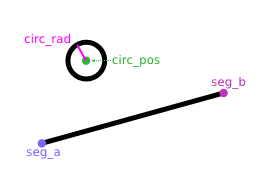
\includegraphics[height=35mm]{circle_intersect.png}
    \end{center}
    \item <3->{Ajuster le mouvement des objets}
    \end{itemize}
\end{frame}

\begin{frame}[fragile]
  \frametitle<1->{\center{Les scores}}
    \begin{column}
      \begin{itemize}
        \item <1->{Le nombre de pièces accumulées détermine le score}
        \item <2->{Une classe spécifique pour modéliser les scores:}
        \begin{lstlisting}[language=java]
          public class Score implements Serializable {
          private int rank, value;
          private double lat, lng; ...
        \end{lstlisting}
      \end{itemize}
    \end{column}
    \begin{column}
      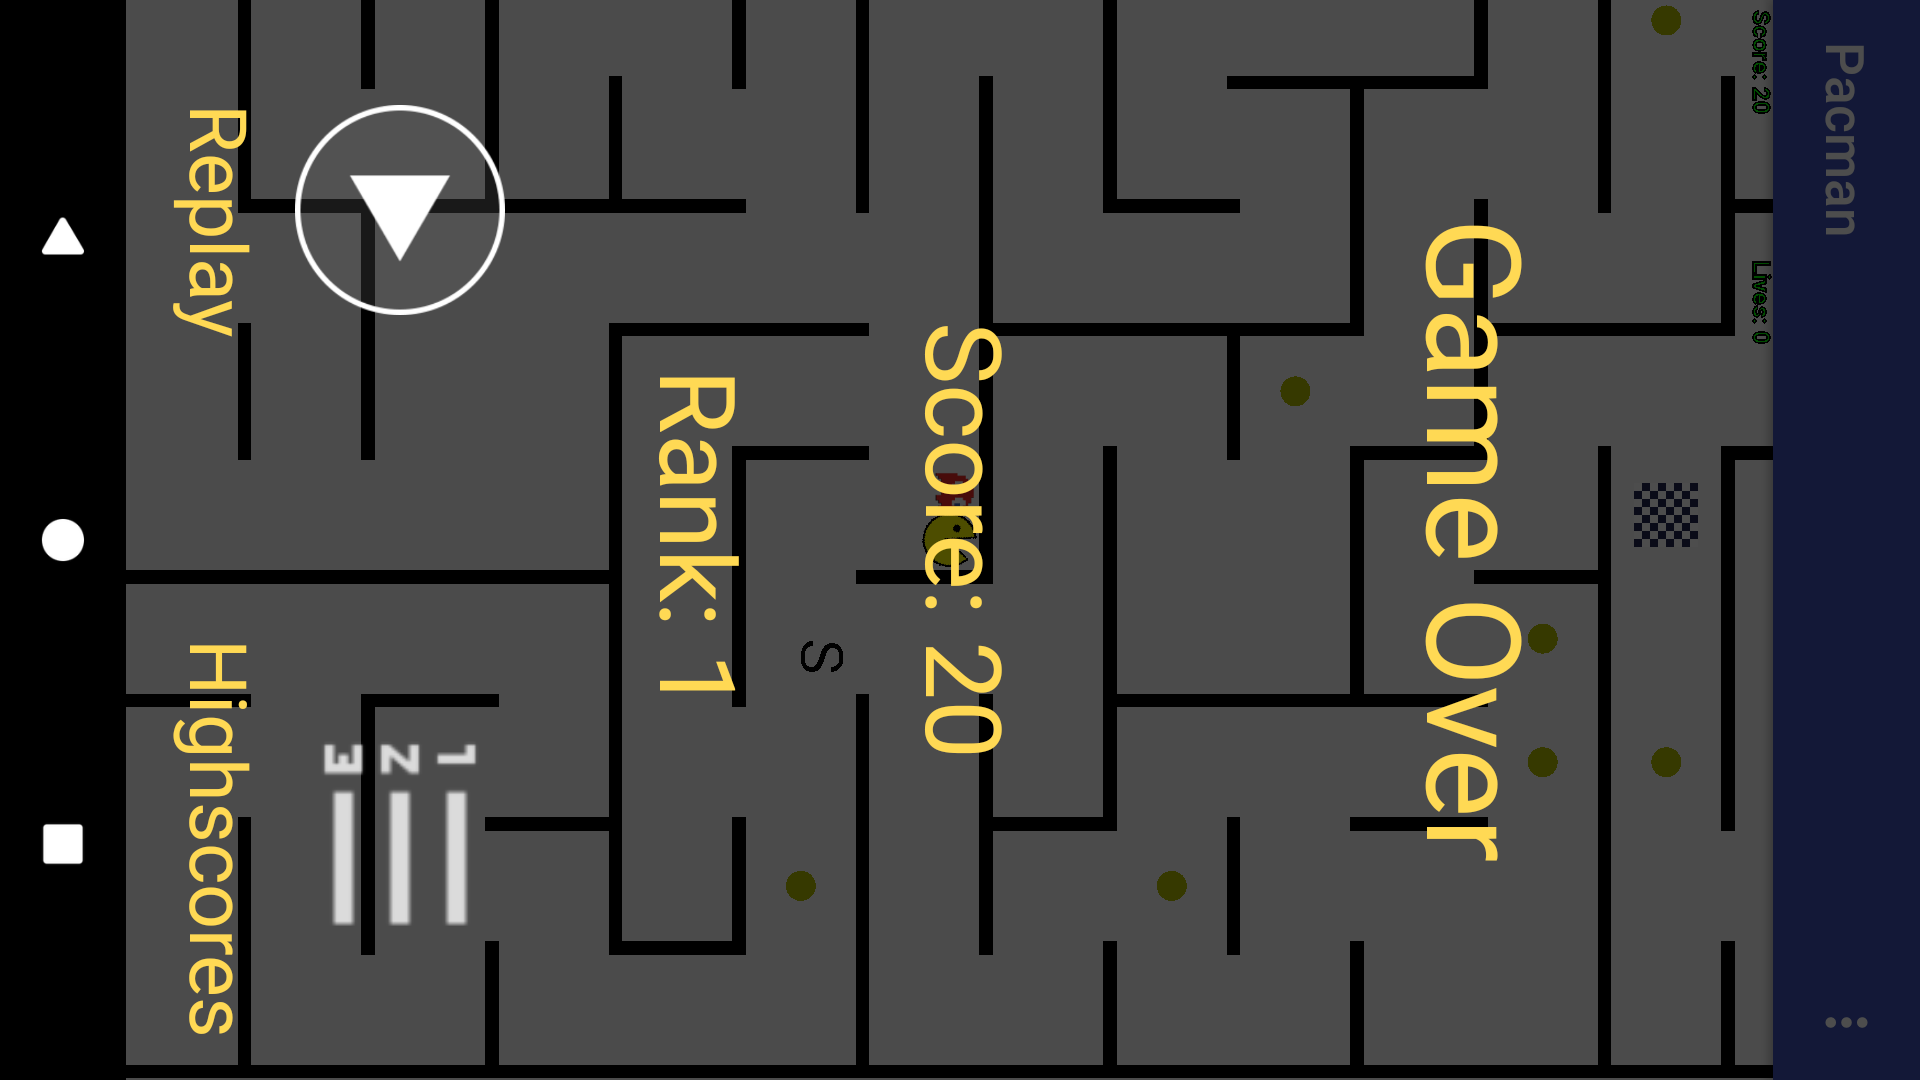
\includegraphics[height=5cm]{game_over.png}
    \end{column}
    \begin{itemize}
      \item <3->{Une activité pour l'affichage d'une liste de scores}
      \item <2->{Gestion de la persistance avec une base de données SQLite
    \end{itemize}
\end{frame}

\begin{frame}[fragile]
  \frametitle<1->{Liste de scores}
  \begin{itemize}
    \item <1->{La liste est accessible à de multiples endroits: menu du jeu, menu principal, ecran de game over}
    \item <2->{La vue \enquote{ListView} pour afficher une liste}
    \begin{center}
      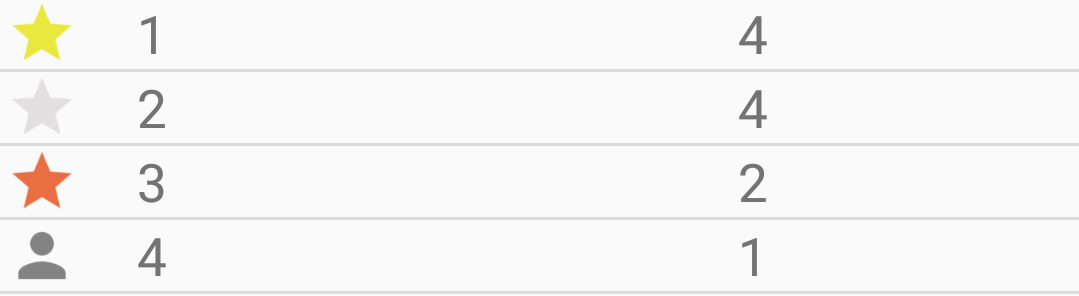
\includegraphics[height=15mm]{scores_list.png}
    \end{center}
    \item <3->{Un \enquote{ArrayAdapter} pour réaliser l'interface entre les scores et la vue}% parler du cell_layout
    \item <4->{La méthode getView pour afficher un score à une position spécifique dans la liste}
    % parler du score surligné (highlight)
    \begin{lstlisting}[language=java]
      Score score = getItem(position);
      int rank = score.getRank();
      int value = score.getValue();
      rankView.setText( String.valueOf(rank) );
      scoreView.setText( String.valueOf( value ) );
      switch(rank) { /* selection de l'image en fonction du rang... */ }
      return cellView;
    \end{lstlisting}
  \end{itemize}
\end{frame}

\begin{frame}[fragile]
  \frametitle<1->{Persistance}
    \begin{itemize}
    \item <1->{Conservation des scores avec une base de données SQLite:}
    \begin{lstlisting}[language=java]
      public class DBManager extends SQLiteOpenHelper {
        ...
        public void onCreate(SQLiteDatabase db) { 
          db.execSQL("create table scores (" +
            SCORES_COLUMN_ID+" integer primary key autoincrement, " +
            SCORES_COLUMN_VALUE+" integer, " +
            SCORES_COLUMN_LATITUDE+" real, " +
            SCORES_COLUMN_LONGITUDE+" real)"
        );}
    \end{lstlisting}
    % oncreate / onUpgrade / onOpen
    \item <2->{\enquote{getWritableDatabase} et \enquote{getReadableDatabase} créent, ouvrent ou mettent à jour la base}
    \item <3->{Un fichier \enquote{ScoresDB.db} est crée dans un dossier protégé}
    \item <4->{Permet d'interroger la base avec des requêtes SQL simples} % getAllScore et getRank par ex
    \end{itemize}
\end{frame}

\begin{frame}[fragile]
  \frametitle<1->{Localisation du téléphone}
    \begin{itemize} % parler de la classe SingleShot...
    \item <1->{Récupérer une seule fois la position} % parler de ACCURACY_COARCE et ACCURACY_FINE
    \item <2->{Utiliser la méthode \enquote{requestSingleUpdate} de la classe \enquote{LocationManager}}
    \begin{lstlisting}[language=java]
       locationManager.requestSingleUpdate( criteria, new MyLocationListener( callback ), null );

       private static class MyLocationListener implements LocationListener { ...
         public void onLocationChanged( Location location ) {
          callback.onNewLocationAvailable( new Double[] {location.getLatitude(), location.getLongitude()} 
          );}
    \end{lstlisting}
    \item <3->{Prendre en compte les autorisations et la latence} % parler du gps et du reseau (enabled...)
    \item <3->{Transmission des coordonnées avec la méthode \enquote{putExtra} de la classe \enquote{Intent}} % parler du bundle
    \end{itemize}
\end{frame}

\begin{frame}[fragile]
  \frametitle<1->{La carte} % parler de l'accès à la carte (scores => click => transmission => layout...)
    \begin{itemize}
    \item <1->{Utilisation de l'API Google Map}% simple fragment pour le layout
    \item <2->{Un simple fragment pour le layout:}
    \begin{center}
      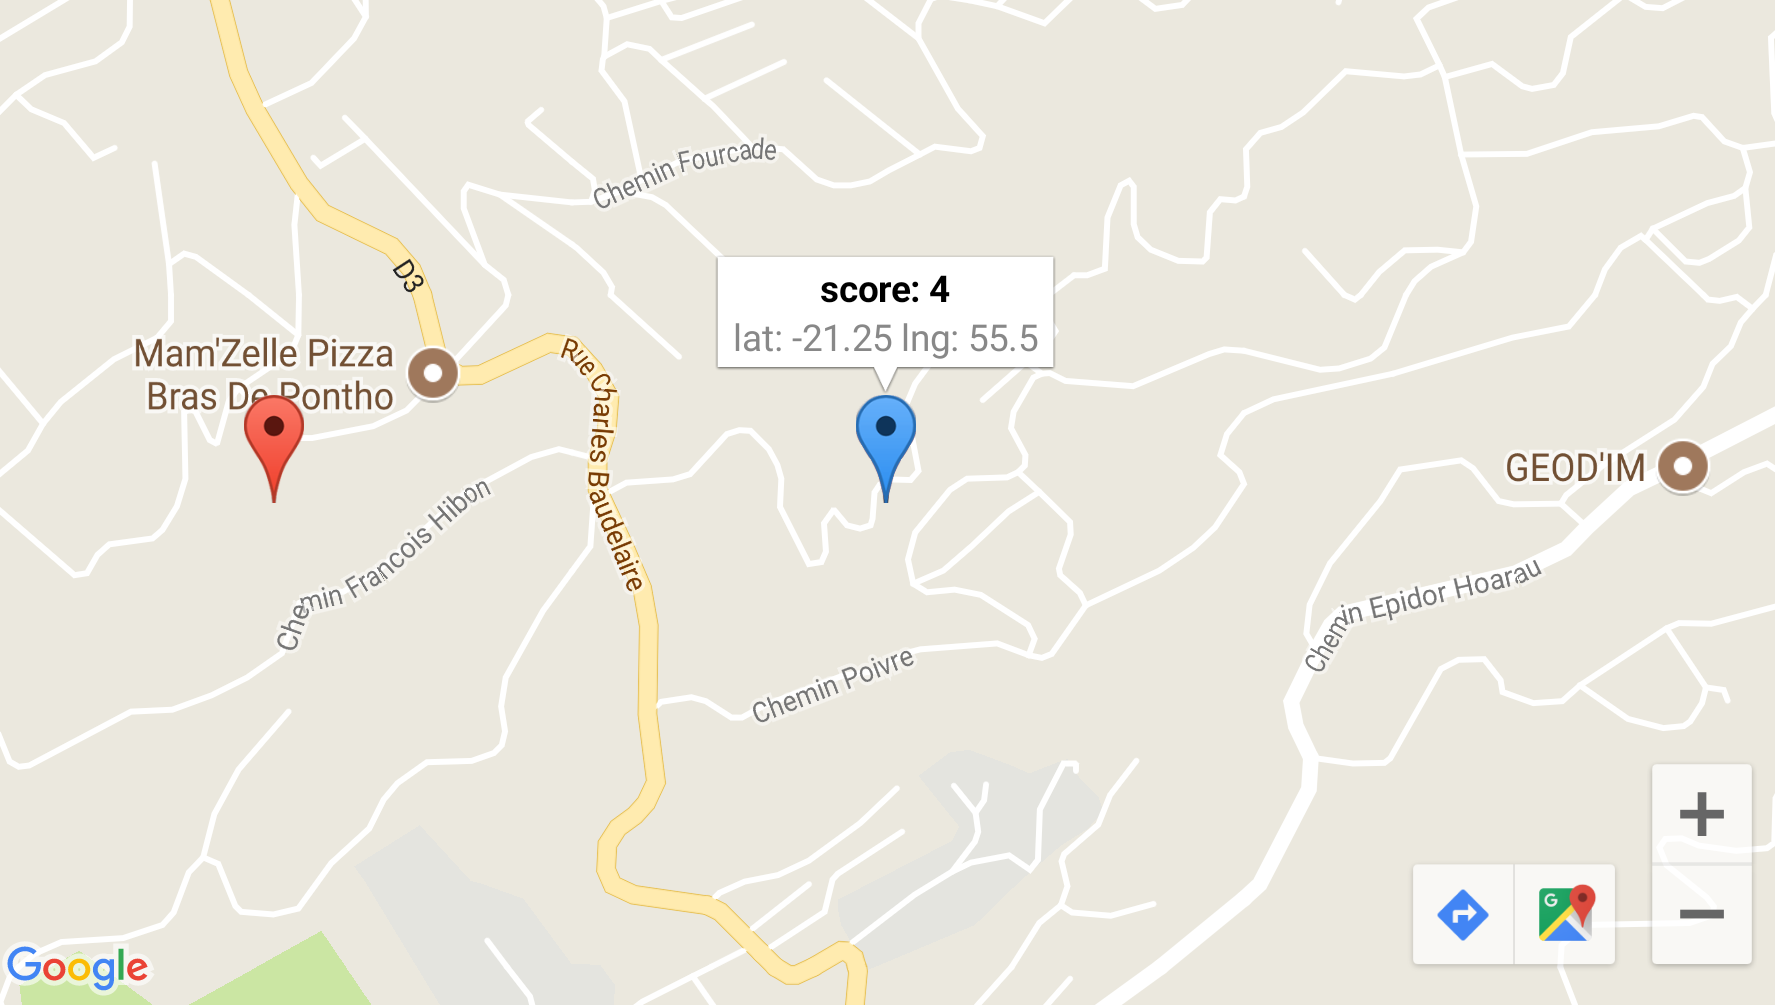
\includegraphics[height=25mm]{map_marker.png}
    \end{center}
    \item <3->{Récupération des coordonnées des scores}
    \item <4->{\enquote{onMapReady} pour l'affichage des marqueurs de position}
    \begin{lstlisting}[language=java]
    int centerScoreRank = centerScore.getRank();
    for(Score score: scores_array){
        mMap.addMarker( createMarker( score, score.getRank()==centerScoreRank ) );
    }
    LatLng centerLatLng = new LatLng( centerScore.getLatitude(), centerScore.getLongitude() );
    mMap.animateCamera( CameraUpdateFactory.newLatLngZoom( centerLatLng, 11 ) );
    \end{lstlisting} % parler des MarkerOptions dans createMarker(...) 
    \end{itemize}
\end{frame}

\begin{frame}[fragile]
  \frametitle<1->{Les sons}
    \begin{itemize}%parler de la libération des ressources
    \item <1->{Utilisation de la classe MediaPlayer}% parler du wrapper AudioPlayer
    \item <2->{Lecture d'un fichier du dossier \enquote{Assets}}% parler d'assets vs res/raw
      \begin{lstlisting}[language=java]
        player = new MediaPlayer();
        player.setVolume(volume, volume);
        player.setDataSource(afd.getFileDescriptor(), afd.getStartOffset(), afd.getLength());
        player.setLooping(loop);
        player.prepare();
        player.setOnCompletionListener( new MediaPlayer.OnCompletionListener() {
          public void onCompletion( MediaPlayer mp ) {
            stopPlayer();
          }});
      \end{lstlisting} %parler de startPlayer / stopPlayer
    \item <2->{Gestion de la libération des ressources} % parler de onPause / on Resume / onDestroy
   \end{itemize}
\end{frame}

\begin{frame}
  \frametitle<1->{Conclusion}
    \begin{itemize}
      \item <1->{Création d'un jeu simple intégrant un modèle physique}%cinématique / coincider forme geom => sprites
      \item <2->{Un ensemble d'activités et d'objets qui coopèrent}% chacune participe à une fonctionnalit de l'appli
      \item <3->{Utilisation des fonctionnalités du téléphone: capteurs, services...}%position(network + gps) / accel / son
      \item <4->{Un jeu perfectible}% deplacement des ennemis / niveaux / différent type d'ennemis / fuite etc...
   \end{itemize}
\end{frame}

\end{document}
